\scanpage{5}
est incident au côté géométrique $D(s',s'')$
\uline{ssi} $s$ est incident au côté combinatoire, i.e.
$s=s'$ ou $s=s''$\,; ceci implique bien entendu
que les côtés géom corr. 1-1 aux côtés
combinatoires. On verra que les polygônes
réguliers (\unsure{même|mê} sans la condition unimodulaire)
sont \inserted{\unsure{néc|sic|aussi}} propres.

\figure{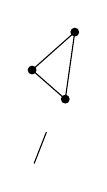
\begin{tikzpicture}[x=.86cm,y=.86cm]
\draw (0,.47)--(.63,1.03)--(.49,.04)--cycle;
\foreach \p in {(0,.47),(.63,1.03),(.49,.04)}{\fill \p circle (1.6pt);}
\draw (.21,-.45)--(.03,-.91);
\end{tikzpicture}}
La condition d'unicité dans la définition
du polygône régulier équivaut évidemment
à dire que $S$ engendre aff\textsuperscript{t} $E$, ou encore
que $S$ n'est pas \deleted{sur} \inserted{contenu dans} une droite. Il
revient au $=$ \deleted{que} de dire que
trois sommets consécutifs $s_0,s_1,s_2$ \uline{donnés}
sont non alignés [suffisance claire, pour la
nécessité on voit que si $d_0=D(s_0,s_1)$, on aurait
sinon \deleted{\unsure{$d$|$d_1$}} $d_0=u(d_0)$ [$us_0=s_1,\ldots$], donc
tous les $d_i$ égaux puisque $u$ transitif
sur l'ens des côtés, absurde \ldots].

% slanted
\margin{p\textsuperscript{t} de vue \unsure{voisin|inverse} fixer $\Pi$ (le ``schéma combinatoire'') \unsure{parler des|pour des|plutôt des} polygônes et \unsure{non après|ns après} \unsure{réguliers|s'agiter|épinglés}.}
Épinglage d'un polygône géom. par
un pol. comb $\Pi$ -- un polygône
géom. $\Pi$ épinglé\,: revient à la donnée
d'un couple \deleted{\unsure{$(S,\varphi)$|$(P$}} $(\Pi,\varphi)$, $\Pi=(S,\omega)$
polyg comb, $\varphi:S\longrightarrow E$ application injective
% archive sheet number: 4

